% Options for packages loaded elsewhere
\PassOptionsToPackage{unicode}{hyperref}
\PassOptionsToPackage{hyphens}{url}
%
\documentclass[
]{book}
\usepackage{amsmath,amssymb}
\usepackage{lmodern}
\usepackage{ifxetex,ifluatex}
\ifnum 0\ifxetex 1\fi\ifluatex 1\fi=0 % if pdftex
  \usepackage[T1]{fontenc}
  \usepackage[utf8]{inputenc}
  \usepackage{textcomp} % provide euro and other symbols
\else % if luatex or xetex
  \usepackage{unicode-math}
  \defaultfontfeatures{Scale=MatchLowercase}
  \defaultfontfeatures[\rmfamily]{Ligatures=TeX,Scale=1}
\fi
% Use upquote if available, for straight quotes in verbatim environments
\IfFileExists{upquote.sty}{\usepackage{upquote}}{}
\IfFileExists{microtype.sty}{% use microtype if available
  \usepackage[]{microtype}
  \UseMicrotypeSet[protrusion]{basicmath} % disable protrusion for tt fonts
}{}
\makeatletter
\@ifundefined{KOMAClassName}{% if non-KOMA class
  \IfFileExists{parskip.sty}{%
    \usepackage{parskip}
  }{% else
    \setlength{\parindent}{0pt}
    \setlength{\parskip}{6pt plus 2pt minus 1pt}}
}{% if KOMA class
  \KOMAoptions{parskip=half}}
\makeatother
\usepackage{xcolor}
\IfFileExists{xurl.sty}{\usepackage{xurl}}{} % add URL line breaks if available
\IfFileExists{bookmark.sty}{\usepackage{bookmark}}{\usepackage{hyperref}}
\hypersetup{
  pdftitle={Psy 300 Statistics Workbook},
  pdfauthor={James Van Slyke},
  hidelinks,
  pdfcreator={LaTeX via pandoc}}
\urlstyle{same} % disable monospaced font for URLs
\usepackage{color}
\usepackage{fancyvrb}
\newcommand{\VerbBar}{|}
\newcommand{\VERB}{\Verb[commandchars=\\\{\}]}
\DefineVerbatimEnvironment{Highlighting}{Verbatim}{commandchars=\\\{\}}
% Add ',fontsize=\small' for more characters per line
\usepackage{framed}
\definecolor{shadecolor}{RGB}{248,248,248}
\newenvironment{Shaded}{\begin{snugshade}}{\end{snugshade}}
\newcommand{\AlertTok}[1]{\textcolor[rgb]{0.94,0.16,0.16}{#1}}
\newcommand{\AnnotationTok}[1]{\textcolor[rgb]{0.56,0.35,0.01}{\textbf{\textit{#1}}}}
\newcommand{\AttributeTok}[1]{\textcolor[rgb]{0.77,0.63,0.00}{#1}}
\newcommand{\BaseNTok}[1]{\textcolor[rgb]{0.00,0.00,0.81}{#1}}
\newcommand{\BuiltInTok}[1]{#1}
\newcommand{\CharTok}[1]{\textcolor[rgb]{0.31,0.60,0.02}{#1}}
\newcommand{\CommentTok}[1]{\textcolor[rgb]{0.56,0.35,0.01}{\textit{#1}}}
\newcommand{\CommentVarTok}[1]{\textcolor[rgb]{0.56,0.35,0.01}{\textbf{\textit{#1}}}}
\newcommand{\ConstantTok}[1]{\textcolor[rgb]{0.00,0.00,0.00}{#1}}
\newcommand{\ControlFlowTok}[1]{\textcolor[rgb]{0.13,0.29,0.53}{\textbf{#1}}}
\newcommand{\DataTypeTok}[1]{\textcolor[rgb]{0.13,0.29,0.53}{#1}}
\newcommand{\DecValTok}[1]{\textcolor[rgb]{0.00,0.00,0.81}{#1}}
\newcommand{\DocumentationTok}[1]{\textcolor[rgb]{0.56,0.35,0.01}{\textbf{\textit{#1}}}}
\newcommand{\ErrorTok}[1]{\textcolor[rgb]{0.64,0.00,0.00}{\textbf{#1}}}
\newcommand{\ExtensionTok}[1]{#1}
\newcommand{\FloatTok}[1]{\textcolor[rgb]{0.00,0.00,0.81}{#1}}
\newcommand{\FunctionTok}[1]{\textcolor[rgb]{0.00,0.00,0.00}{#1}}
\newcommand{\ImportTok}[1]{#1}
\newcommand{\InformationTok}[1]{\textcolor[rgb]{0.56,0.35,0.01}{\textbf{\textit{#1}}}}
\newcommand{\KeywordTok}[1]{\textcolor[rgb]{0.13,0.29,0.53}{\textbf{#1}}}
\newcommand{\NormalTok}[1]{#1}
\newcommand{\OperatorTok}[1]{\textcolor[rgb]{0.81,0.36,0.00}{\textbf{#1}}}
\newcommand{\OtherTok}[1]{\textcolor[rgb]{0.56,0.35,0.01}{#1}}
\newcommand{\PreprocessorTok}[1]{\textcolor[rgb]{0.56,0.35,0.01}{\textit{#1}}}
\newcommand{\RegionMarkerTok}[1]{#1}
\newcommand{\SpecialCharTok}[1]{\textcolor[rgb]{0.00,0.00,0.00}{#1}}
\newcommand{\SpecialStringTok}[1]{\textcolor[rgb]{0.31,0.60,0.02}{#1}}
\newcommand{\StringTok}[1]{\textcolor[rgb]{0.31,0.60,0.02}{#1}}
\newcommand{\VariableTok}[1]{\textcolor[rgb]{0.00,0.00,0.00}{#1}}
\newcommand{\VerbatimStringTok}[1]{\textcolor[rgb]{0.31,0.60,0.02}{#1}}
\newcommand{\WarningTok}[1]{\textcolor[rgb]{0.56,0.35,0.01}{\textbf{\textit{#1}}}}
\usepackage{longtable,booktabs,array}
\usepackage{calc} % for calculating minipage widths
% Correct order of tables after \paragraph or \subparagraph
\usepackage{etoolbox}
\makeatletter
\patchcmd\longtable{\par}{\if@noskipsec\mbox{}\fi\par}{}{}
\makeatother
% Allow footnotes in longtable head/foot
\IfFileExists{footnotehyper.sty}{\usepackage{footnotehyper}}{\usepackage{footnote}}
\makesavenoteenv{longtable}
\usepackage{graphicx}
\makeatletter
\def\maxwidth{\ifdim\Gin@nat@width>\linewidth\linewidth\else\Gin@nat@width\fi}
\def\maxheight{\ifdim\Gin@nat@height>\textheight\textheight\else\Gin@nat@height\fi}
\makeatother
% Scale images if necessary, so that they will not overflow the page
% margins by default, and it is still possible to overwrite the defaults
% using explicit options in \includegraphics[width, height, ...]{}
\setkeys{Gin}{width=\maxwidth,height=\maxheight,keepaspectratio}
% Set default figure placement to htbp
\makeatletter
\def\fps@figure{htbp}
\makeatother
\setlength{\emergencystretch}{3em} % prevent overfull lines
\providecommand{\tightlist}{%
  \setlength{\itemsep}{0pt}\setlength{\parskip}{0pt}}
\setcounter{secnumdepth}{5}
\usepackage{booktabs}
\ifluatex
  \usepackage{selnolig}  % disable illegal ligatures
\fi
\usepackage[]{natbib}
\bibliographystyle{apalike}

\title{Psy 300 Statistics Workbook}
\author{James Van Slyke}
\date{2021-06-01}

\begin{document}
\maketitle

{
\setcounter{tocdepth}{1}
\tableofcontents
}
\hypertarget{introduction}{%
\chapter{Introduction}\label{introduction}}

This is a workbook of various examples of statistical analyis to explore psychology experiments.The workbook uses R for all it's calculations and R Studio is assumed to be the program used for those calculations.

If you have not downloaded R and R Studio you can go to these websites

R

R Studio

On the left you'll see examples from each of the primary statisitcal analyses used in this class. Two other books will be important to use as references.

R for Data Science

Using R to something something Psychology

\hypertarget{independent-t-test}{%
\chapter{Independent t-test}\label{independent-t-test}}

Independent t-test example

\begin{enumerate}
\def\labelenumi{\arabic{enumi}.}
\tightlist
\item
  First Step, upload dataset from SPSS
\item
  Get data set named ``Invisibility'' from SPSS datasets
\item
  Use \emph{import dataset} tool under the environment tab
\item
  Find file called \emph{invisibility.sav}
\end{enumerate}

\begin{Shaded}
\begin{Highlighting}[]
\FunctionTok{library}\NormalTok{(haven)}
\NormalTok{Invisibility }\OtherTok{\textless{}{-}} \FunctionTok{read\_sav}\NormalTok{(}\StringTok{"Invisibility.sav"}\NormalTok{)}
\FunctionTok{View}\NormalTok{(Invisibility)}
\end{Highlighting}
\end{Shaded}

Inspect variables

\begin{Shaded}
\begin{Highlighting}[]
\NormalTok{Invisibility}\SpecialCharTok{$}\NormalTok{Cloak}
\NormalTok{Invisibility}\SpecialCharTok{$}\NormalTok{Mischief}
\end{Highlighting}
\end{Shaded}

Create bar graph to examine data
First step is to create a dataset with your descriptive variables
We'll use the dplyr package to do this, which is part of tidyverse

\begin{Shaded}
\begin{Highlighting}[]
\FunctionTok{library}\NormalTok{(dplyr)}
\NormalTok{Invis\_Descriptives }\OtherTok{\textless{}{-}}\NormalTok{ Invisibility }\SpecialCharTok{\%\textgreater{}\%}
  \FunctionTok{group\_by}\NormalTok{(Cloak) }\SpecialCharTok{\%\textgreater{}\%}
  \FunctionTok{summarize}\NormalTok{(}\AttributeTok{n =} \FunctionTok{n}\NormalTok{(),}
            \AttributeTok{mean =} \FunctionTok{mean}\NormalTok{(Mischief),}
            \AttributeTok{sd =} \FunctionTok{sd}\NormalTok{(Mischief),}
            \AttributeTok{se =}\NormalTok{ sd }\SpecialCharTok{/} \FunctionTok{sqrt}\NormalTok{(n),}
            \AttributeTok{ci =} \FunctionTok{qt}\NormalTok{(}\FloatTok{0.975}\NormalTok{, }\AttributeTok{df =}\NormalTok{ n }\SpecialCharTok{{-}} \DecValTok{1}\NormalTok{) }\SpecialCharTok{*}\NormalTok{ sd }\SpecialCharTok{/} \FunctionTok{sqrt}\NormalTok{(n))}
\end{Highlighting}
\end{Shaded}

First let's make a simple graph with just the basics

\begin{Shaded}
\begin{Highlighting}[]
\FunctionTok{ggplot}\NormalTok{(Invis\_Descriptives, }
       \FunctionTok{aes}\NormalTok{(}\AttributeTok{x =}\NormalTok{ Cloak, }
           \AttributeTok{y =}\NormalTok{ mean)) }\SpecialCharTok{+}
  \FunctionTok{geom\_bar}\NormalTok{(}\AttributeTok{stat =} \StringTok{"identity"}\NormalTok{)}
\end{Highlighting}
\end{Shaded}

Next let's add error bars

\begin{Shaded}
\begin{Highlighting}[]
\FunctionTok{ggplot}\NormalTok{(Invis\_Descriptives, }
       \FunctionTok{aes}\NormalTok{(}\AttributeTok{x =}\NormalTok{ Cloak, }
           \AttributeTok{y =}\NormalTok{ mean)) }\SpecialCharTok{+}
  \FunctionTok{geom\_bar}\NormalTok{(}\AttributeTok{stat =} \StringTok{"identity"}\NormalTok{) }\SpecialCharTok{+}
  \FunctionTok{geom\_errorbar}\NormalTok{(}\FunctionTok{aes}\NormalTok{(}\AttributeTok{ymin=}\NormalTok{mean}\SpecialCharTok{{-}}\NormalTok{ci,}
                    \AttributeTok{ymax=}\NormalTok{mean}\SpecialCharTok{+}\NormalTok{ci))}
\end{Highlighting}
\end{Shaded}

We can add in labels to improve the look of our chart.
We've added labels to our factor variable and labels for
the title and x and y variables.

\begin{Shaded}
\begin{Highlighting}[]
\FunctionTok{ggplot}\NormalTok{(Invis\_Descriptives, }
       \FunctionTok{aes}\NormalTok{(}\AttributeTok{x =} \FunctionTok{factor}\NormalTok{(Cloak, }\AttributeTok{labels=}\FunctionTok{c}\NormalTok{(}\StringTok{"No Cloak"}\NormalTok{, }\StringTok{"Cloak"}\NormalTok{)),}
           \AttributeTok{y =}\NormalTok{ mean)) }\SpecialCharTok{+}
  \FunctionTok{geom\_bar}\NormalTok{(}\AttributeTok{stat =} \StringTok{"identity"}\NormalTok{) }\SpecialCharTok{+}
  \FunctionTok{geom\_errorbar}\NormalTok{(}\FunctionTok{aes}\NormalTok{(}\AttributeTok{ymin=}\NormalTok{mean}\SpecialCharTok{{-}}\NormalTok{ci,}
                    \AttributeTok{ymax=}\NormalTok{mean}\SpecialCharTok{+}\NormalTok{ci)) }\SpecialCharTok{+}
  \FunctionTok{labs}\NormalTok{(}\AttributeTok{title =} \StringTok{"Mean Number of Mischievious Acts with or without Cloak"}\NormalTok{, }
       \AttributeTok{y=}\StringTok{"Mean Number of Mischievious Acts"}\NormalTok{, }\AttributeTok{x=}\StringTok{"Were They Wearing a Cloak?"}\NormalTok{)}
\end{Highlighting}
\end{Shaded}

Next let's add some color to our chart

\begin{Shaded}
\begin{Highlighting}[]
\FunctionTok{ggplot}\NormalTok{(Invis\_Descriptives, }
       \FunctionTok{aes}\NormalTok{(}\AttributeTok{x =} \FunctionTok{factor}\NormalTok{(Cloak, }\AttributeTok{labels=}\FunctionTok{c}\NormalTok{(}\StringTok{"No Cloak"}\NormalTok{, }\StringTok{"Cloak"}\NormalTok{)),}
           \AttributeTok{y =}\NormalTok{ mean)) }\SpecialCharTok{+}
  \FunctionTok{theme\_minimal}\NormalTok{() }\SpecialCharTok{+}
  \FunctionTok{geom\_bar}\NormalTok{(}\AttributeTok{stat =} \StringTok{"identity"}\NormalTok{, }\AttributeTok{fill=}\StringTok{"cornflowerblue"}\NormalTok{) }\SpecialCharTok{+}
  \FunctionTok{geom\_errorbar}\NormalTok{(}\FunctionTok{aes}\NormalTok{(}\AttributeTok{ymin=}\NormalTok{mean}\SpecialCharTok{{-}}\NormalTok{ci,}
                    \AttributeTok{ymax=}\NormalTok{mean}\SpecialCharTok{+}\NormalTok{ci), }\AttributeTok{width=}\NormalTok{.}\DecValTok{3}\NormalTok{, }\AttributeTok{size=}\DecValTok{1}\NormalTok{) }\SpecialCharTok{+}
  \FunctionTok{labs}\NormalTok{(}\AttributeTok{title =} \StringTok{"Mean Number of Mischievious Acts with or without Cloak"}\NormalTok{, }
       \AttributeTok{y=}\StringTok{"Mean Number of Mischievious Acts"}\NormalTok{, }\AttributeTok{x=}\StringTok{"Were They Wearing a Cloak?"}\NormalTok{)}
\end{Highlighting}
\end{Shaded}

Based on the graph, it looks like there is a difference between the groups Let's run a t test to make sure

\begin{Shaded}
\begin{Highlighting}[]
\FunctionTok{t.test}\NormalTok{(Mischief }\SpecialCharTok{\textasciitilde{}}\NormalTok{ Cloak, }\AttributeTok{data =}\NormalTok{ Invisibility)}
\end{Highlighting}
\end{Shaded}

List the effect size as well
Cohen's d - Subtract the means from each other and
divide by the standard deviation of the control group

\begin{Shaded}
\begin{Highlighting}[]
\NormalTok{Cohens\_d }\OtherTok{\textless{}{-}}\NormalTok{ (}\FloatTok{5.00{-}3.75}\NormalTok{)}\SpecialCharTok{/}\FloatTok{1.91}
\end{Highlighting}
\end{Shaded}

Write out conclusion

\emph{On average, participants given a cloak of invisibility engaged in
more acts of mischief (M = 5, SE = 0.48), than those not given a
cloak (M = 3.75, SE = 0.55). This difference, 1.25, 95\% CI{[}-2.76, 0.26{]},
was not significant t(21.54) = −1.71, p = 0.101; however, it did
represent a medium-sized effect d = 0.65.}

Steps to writing results

\begin{enumerate}
\def\labelenumi{\arabic{enumi}.}
\tightlist
\item
  Write out the means and include standard error
\item
  Write out the difference between the means (Subtract the sample means) and the confidence intervals for the difference
\item
  t(df)= t score, p value, Cohen's d
\end{enumerate}

\hypertarget{paired-samples-t-test}{%
\chapter{Paired samples t-test}\label{paired-samples-t-test}}

Check out dataset
View Spreadsheet

\begin{Shaded}
\begin{Highlighting}[]
\FunctionTok{View}\NormalTok{(ch14ds1)}
\end{Highlighting}
\end{Shaded}

Info on dataset
Research hypothesis -

View in Console

\begin{Shaded}
\begin{Highlighting}[]
\NormalTok{ch14ds1}
\end{Highlighting}
\end{Shaded}

View Descriptive Statistics

\begin{Shaded}
\begin{Highlighting}[]
\FunctionTok{summary}\NormalTok{(ch14ds1)}
\end{Highlighting}
\end{Shaded}

Graph data using a boxplot to get a first glimpse

\begin{Shaded}
\begin{Highlighting}[]
\FunctionTok{boxplot}\NormalTok{(ch14ds1}\SpecialCharTok{$}\NormalTok{Pretest, ch14ds1}\SpecialCharTok{$}\NormalTok{Posttest)}
\end{Highlighting}
\end{Shaded}

Run the t test for paired samples (also sometimes called the Dependent t test)

\begin{Shaded}
\begin{Highlighting}[]
\FunctionTok{t.test}\NormalTok{(ch14ds1}\SpecialCharTok{$}\NormalTok{Posttest, ch14ds1}\SpecialCharTok{$}\NormalTok{Pretest, }\AttributeTok{paired =} \ConstantTok{TRUE}\NormalTok{)}
\end{Highlighting}
\end{Shaded}

This time let's use a ggplot to make a better looking bar graph. Check out the format of the data

\begin{Shaded}
\begin{Highlighting}[]
\NormalTok{ch14ds1}
\end{Highlighting}
\end{Shaded}

The data is set up for a paired t test, so it includes 2 numeric variables This is a proiblem because we are missing our a single factor variable to describe our two bars (i.e.~pre and post test).
Thus, we are going to create a second dataset that has a factor (``group'') and numeric (``Test'') variable. Notice I'm creating a new dataframe, calling it ``TestData''. I'm creating the factor variable from scratch using the ``rep'' repeat function and then adding together the Pre and Post Test scores into a single number variable.

\begin{Shaded}
\begin{Highlighting}[]
\NormalTok{TestData }\OtherTok{\textless{}{-}} \FunctionTok{data.frame}\NormalTok{(}
            \AttributeTok{group=} \FunctionTok{rep}\NormalTok{(}\FunctionTok{c}\NormalTok{(}\StringTok{"Pretest"}\NormalTok{, }\StringTok{"Posttest"}\NormalTok{), }\AttributeTok{each=}\DecValTok{25}\NormalTok{),}
            \AttributeTok{Test =} \FunctionTok{c}\NormalTok{(ch14ds1}\SpecialCharTok{$}\NormalTok{Pretest, ch14ds1}\SpecialCharTok{$}\NormalTok{Posttest)}
\NormalTok{            )}
\end{Highlighting}
\end{Shaded}

Next, I'll find my descriptive statistics for this dataset

\begin{Shaded}
\begin{Highlighting}[]
\FunctionTok{library}\NormalTok{(dplyr)}
\NormalTok{Test\_Descriptives }\OtherTok{\textless{}{-}}\NormalTok{ TestData }\SpecialCharTok{\%\textgreater{}\%}
  \FunctionTok{group\_by}\NormalTok{(group) }\SpecialCharTok{\%\textgreater{}\%}
  \FunctionTok{summarize}\NormalTok{(}\AttributeTok{n =} \FunctionTok{n}\NormalTok{(),}
            \AttributeTok{mean =} \FunctionTok{mean}\NormalTok{(Test),}
            \AttributeTok{sd =} \FunctionTok{sd}\NormalTok{(Test),}
            \AttributeTok{se =}\NormalTok{ sd }\SpecialCharTok{/} \FunctionTok{sqrt}\NormalTok{(n),}
            \AttributeTok{ci =} \FunctionTok{qt}\NormalTok{(}\FloatTok{0.975}\NormalTok{, }\AttributeTok{df =}\NormalTok{ n }\SpecialCharTok{{-}} \DecValTok{1}\NormalTok{) }\SpecialCharTok{*}\NormalTok{ sd }\SpecialCharTok{/} \FunctionTok{sqrt}\NormalTok{(n))}
\end{Highlighting}
\end{Shaded}

Check your descriptives, make sure they turned out ok.

\begin{Shaded}
\begin{Highlighting}[]
\NormalTok{Test\_Descriptives}
\end{Highlighting}
\end{Shaded}

Finally, create a basic bar graph

\begin{Shaded}
\begin{Highlighting}[]
\FunctionTok{ggplot}\NormalTok{(Test\_Descriptives, }
       \FunctionTok{aes}\NormalTok{(}\AttributeTok{x =}\NormalTok{ group, }
           \AttributeTok{y =}\NormalTok{ mean)) }\SpecialCharTok{+}
  \FunctionTok{geom\_bar}\NormalTok{(}\AttributeTok{stat =} \StringTok{"identity"}\NormalTok{)}
\end{Highlighting}
\end{Shaded}

Then let's add in some error bars with the geom\_errorbar function

\begin{Shaded}
\begin{Highlighting}[]
\FunctionTok{ggplot}\NormalTok{(Test\_Descriptives, }
       \FunctionTok{aes}\NormalTok{(}\AttributeTok{x =}\NormalTok{ group, }
           \AttributeTok{y =}\NormalTok{ mean)) }\SpecialCharTok{+}
  \FunctionTok{geom\_bar}\NormalTok{(}\AttributeTok{stat =} \StringTok{"identity"}\NormalTok{) }\SpecialCharTok{+}
  \FunctionTok{geom\_errorbar}\NormalTok{(}\FunctionTok{aes}\NormalTok{(}\AttributeTok{ymin=}\NormalTok{mean}\SpecialCharTok{{-}}\NormalTok{ci,}
                    \AttributeTok{ymax=}\NormalTok{mean}\SpecialCharTok{+}\NormalTok{ci))}
\end{Highlighting}
\end{Shaded}

Finally, let's make it look really nice

\begin{Shaded}
\begin{Highlighting}[]
\FunctionTok{ggplot}\NormalTok{(Test\_Descriptives, }
       \FunctionTok{aes}\NormalTok{(}\AttributeTok{x =}\NormalTok{ group,}
           \AttributeTok{y =}\NormalTok{ mean)) }\SpecialCharTok{+}
  \FunctionTok{theme\_minimal}\NormalTok{() }\SpecialCharTok{+}
  \FunctionTok{geom\_bar}\NormalTok{(}\AttributeTok{stat =} \StringTok{"identity"}\NormalTok{, }\AttributeTok{fill=}\StringTok{"cornflowerblue"}\NormalTok{) }\SpecialCharTok{+}
  \FunctionTok{geom\_errorbar}\NormalTok{(}\FunctionTok{aes}\NormalTok{(}\AttributeTok{ymin=}\NormalTok{mean}\SpecialCharTok{{-}}\NormalTok{ci,}
                    \AttributeTok{ymax=}\NormalTok{mean}\SpecialCharTok{+}\NormalTok{ci), }\AttributeTok{width=}\NormalTok{.}\DecValTok{3}\NormalTok{, }\AttributeTok{size=}\DecValTok{1}\NormalTok{) }\SpecialCharTok{+}
  \FunctionTok{labs}\NormalTok{(}\AttributeTok{title =} \StringTok{"Change in Performance from Pre to Post Tests"}\NormalTok{, }
       \AttributeTok{y=}\StringTok{"Mean Score"}\NormalTok{, }\AttributeTok{x=}\StringTok{"Tests"}\NormalTok{)}
\end{Highlighting}
\end{Shaded}

You can also flip the columns to make it look cleaner

\begin{Shaded}
\begin{Highlighting}[]
\FunctionTok{ggplot}\NormalTok{(Test\_Descriptives, }
       \FunctionTok{aes}\NormalTok{(}\AttributeTok{x =}\NormalTok{ group,}
           \AttributeTok{y =}\NormalTok{ mean)) }\SpecialCharTok{+}
  \FunctionTok{theme\_minimal}\NormalTok{() }\SpecialCharTok{+}
  \FunctionTok{geom\_bar}\NormalTok{(}\AttributeTok{stat =} \StringTok{"identity"}\NormalTok{, }\AttributeTok{fill=}\StringTok{"cornflowerblue"}\NormalTok{) }\SpecialCharTok{+}
  \FunctionTok{geom\_errorbar}\NormalTok{(}\FunctionTok{aes}\NormalTok{(}\AttributeTok{ymin=}\NormalTok{mean}\SpecialCharTok{{-}}\NormalTok{ci,}
                    \AttributeTok{ymax=}\NormalTok{mean}\SpecialCharTok{+}\NormalTok{ci), }\AttributeTok{width=}\NormalTok{.}\DecValTok{3}\NormalTok{, }\AttributeTok{size=}\DecValTok{1}\NormalTok{) }\SpecialCharTok{+}
  \FunctionTok{labs}\NormalTok{(}\AttributeTok{title =} \StringTok{"Change in Performance from Pre to Post Tests"}\NormalTok{, }
       \AttributeTok{y=}\StringTok{"Mean Score"}\NormalTok{, }\AttributeTok{x=}\StringTok{"Tests"}\NormalTok{) }\SpecialCharTok{+}
  \FunctionTok{scale\_x\_discrete}\NormalTok{(}\AttributeTok{limits=}\FunctionTok{c}\NormalTok{(}\StringTok{"Pretest"}\NormalTok{, }\StringTok{"Posttest"}\NormalTok{))}
\end{Highlighting}
\end{Shaded}

\hypertarget{one-way-anova}{%
\chapter{One Way ANOVA}\label{one-way-anova}}

Practice dataset: How does preschool affect language development?
Three groups that differ by how many hours they spent in preschool per week

Variables
IV = Preschool
DV = Language Development
Language development was measured based on a language development test score

Null Hypothesis: Attendance at preschool has no effect on language development

View Dataset

\begin{Shaded}
\begin{Highlighting}[]
\FunctionTok{View}\NormalTok{(ch15ds1)}
\end{Highlighting}
\end{Shaded}

View in R Console

\begin{Shaded}
\begin{Highlighting}[]
\NormalTok{ch15ds1}
\end{Highlighting}
\end{Shaded}

Let's look at a bar graph of the data first
Step 1 - create table of descriptive statistics

\begin{Shaded}
\begin{Highlighting}[]
\FunctionTok{library}\NormalTok{(dplyr)}
\NormalTok{Preschool\_Descriptives }\OtherTok{\textless{}{-}}\NormalTok{ ch15ds1 }\SpecialCharTok{\%\textgreater{}\%}
  \FunctionTok{group\_by}\NormalTok{(Group) }\SpecialCharTok{\%\textgreater{}\%}
  \FunctionTok{summarize}\NormalTok{(}\AttributeTok{n =} \FunctionTok{n}\NormalTok{(),}
            \AttributeTok{mean =} \FunctionTok{mean}\NormalTok{(Language.Score),}
            \AttributeTok{sd =} \FunctionTok{sd}\NormalTok{(Language.Score),}
            \AttributeTok{se =}\NormalTok{ sd }\SpecialCharTok{/} \FunctionTok{sqrt}\NormalTok{(n),}
            \AttributeTok{ci =} \FunctionTok{qt}\NormalTok{(}\FloatTok{0.975}\NormalTok{, }\AttributeTok{df =}\NormalTok{ n }\SpecialCharTok{{-}} \DecValTok{1}\NormalTok{) }\SpecialCharTok{*}\NormalTok{ sd }\SpecialCharTok{/} \FunctionTok{sqrt}\NormalTok{(n))}
\end{Highlighting}
\end{Shaded}

Check it out

\begin{Shaded}
\begin{Highlighting}[]
\NormalTok{Preschool\_Descriptives}
\end{Highlighting}
\end{Shaded}

Now graph it based on the descriptive statistics

\begin{Shaded}
\begin{Highlighting}[]
\FunctionTok{ggplot}\NormalTok{(Preschool\_Descriptives, }
       \FunctionTok{aes}\NormalTok{(}\AttributeTok{x =}\NormalTok{ Group, }
           \AttributeTok{y =}\NormalTok{ mean)) }\SpecialCharTok{+}
  \FunctionTok{geom\_bar}\NormalTok{(}\AttributeTok{stat =} \StringTok{"identity"}\NormalTok{) }\SpecialCharTok{+}
  \FunctionTok{geom\_errorbar}\NormalTok{(}\FunctionTok{aes}\NormalTok{(}\AttributeTok{ymin=}\NormalTok{mean}\SpecialCharTok{{-}}\NormalTok{ci,}
                    \AttributeTok{ymax=}\NormalTok{mean}\SpecialCharTok{+}\NormalTok{ci))}
\end{Highlighting}
\end{Shaded}

Run your ANOVA
First install Psych package

\begin{Shaded}
\begin{Highlighting}[]
\FunctionTok{library}\NormalTok{(psych)}
\end{Highlighting}
\end{Shaded}

Check out the variables
Psych package uses a different command for this ``describeBy''
Must specify DV and groups

\begin{Shaded}
\begin{Highlighting}[]
\FunctionTok{describeBy}\NormalTok{(ch15ds1}\SpecialCharTok{$}\NormalTok{Language.Score, }\AttributeTok{group =}\NormalTok{ ch15ds1}\SpecialCharTok{$}\NormalTok{Group)}
\end{Highlighting}
\end{Shaded}

Run your ANOVA!
Something new, must save results in an object rather than the results being there automatically

\begin{Shaded}
\begin{Highlighting}[]
\NormalTok{m1 }\OtherTok{\textless{}{-}} \FunctionTok{aov}\NormalTok{(Language.Score}\SpecialCharTok{\textasciitilde{}}\NormalTok{Group, }\AttributeTok{data =}\NormalTok{ ch15ds1)}
\end{Highlighting}
\end{Shaded}

To get ANOVA table must use ``summary'' function

\begin{Shaded}
\begin{Highlighting}[]
\FunctionTok{summary}\NormalTok{(m1)}
\end{Highlighting}
\end{Shaded}

Figure out the effect size - Eta squared
The formula is SSbetween/SSTotal or SSbetween/SSbetween+SSResidual

\begin{Shaded}
\begin{Highlighting}[]
\DecValTok{1133}\SpecialCharTok{/}\NormalTok{(}\DecValTok{1133}\SpecialCharTok{+}\DecValTok{1738}\NormalTok{)}
\end{Highlighting}
\end{Shaded}

Write out conclusion

Number of hours in Preschool had a significant effect on language development, F(2, 27) = 8.799, p = 0.00114, 𝜂2 = 0.39.

Where is the difference? Need to use post hoc tests
TukeyHSD will tell us where the differences are between the individual groups. Run TukeyHSD on saved ANOVA results

\begin{Shaded}
\begin{Highlighting}[]
\FunctionTok{TukeyHSD}\NormalTok{(m1)}
\end{Highlighting}
\end{Shaded}

Finally, write out the whole conclusion
TukeyHSD post hoc tests revealed that 20 hours a week of preschool (M=91.6, SE=1.96) resulted in significantly higher levels of language development in comparison to 5 hours (M=76.6, SE=3.78). This difference, -15 95\% CI{[}-23.90, -6.10{]} was significant with an adjusted p = .0008.

Improve the graph

\begin{Shaded}
\begin{Highlighting}[]
\FunctionTok{ggplot}\NormalTok{(Preschool\_Descriptives, }
       \FunctionTok{aes}\NormalTok{(}\AttributeTok{x =}\NormalTok{ Group, }
           \AttributeTok{y =}\NormalTok{ mean)) }\SpecialCharTok{+}
  \FunctionTok{geom\_bar}\NormalTok{(}\AttributeTok{stat =} \StringTok{"identity"}\NormalTok{) }\SpecialCharTok{+}
  \FunctionTok{geom\_errorbar}\NormalTok{(}\FunctionTok{aes}\NormalTok{(}\AttributeTok{ymin=}\NormalTok{mean}\SpecialCharTok{{-}}\NormalTok{ci,}
                    \AttributeTok{ymax=}\NormalTok{mean}\SpecialCharTok{+}\NormalTok{ci)) }\SpecialCharTok{+}
  \FunctionTok{scale\_x\_discrete}\NormalTok{(}\AttributeTok{limits=}\FunctionTok{c}\NormalTok{(}\StringTok{"5 Hours"}\NormalTok{, }\StringTok{"10 Hours"}\NormalTok{, }\StringTok{"20 Hours"}\NormalTok{))}
\end{Highlighting}
\end{Shaded}

Make it look real nice Clark

\begin{Shaded}
\begin{Highlighting}[]
\FunctionTok{ggplot}\NormalTok{(Preschool\_Descriptives, }
       \FunctionTok{aes}\NormalTok{(}\AttributeTok{x =}\NormalTok{ Group,}
           \AttributeTok{y =}\NormalTok{ mean)) }\SpecialCharTok{+}
  \FunctionTok{theme\_minimal}\NormalTok{() }\SpecialCharTok{+}
  \FunctionTok{geom\_bar}\NormalTok{(}\AttributeTok{stat =} \StringTok{"identity"}\NormalTok{, }\AttributeTok{fill=}\StringTok{"steelblue"}\NormalTok{) }\SpecialCharTok{+}
  \FunctionTok{geom\_errorbar}\NormalTok{(}\FunctionTok{aes}\NormalTok{(}\AttributeTok{ymin=}\NormalTok{mean}\SpecialCharTok{{-}}\NormalTok{ci,}
                    \AttributeTok{ymax=}\NormalTok{mean}\SpecialCharTok{+}\NormalTok{ci), }\AttributeTok{width=}\NormalTok{.}\DecValTok{3}\NormalTok{, }\AttributeTok{size=}\DecValTok{1}\NormalTok{) }\SpecialCharTok{+}
  \FunctionTok{labs}\NormalTok{(}\AttributeTok{title =} \StringTok{"Does Preschool Effect Language Development?"}\NormalTok{, }
       \AttributeTok{y=}\StringTok{"Mean Score on Language Test"}\NormalTok{, }\AttributeTok{x=}\StringTok{"Number of Hours Spent in Preschool"}\NormalTok{) }\SpecialCharTok{+}
  \FunctionTok{scale\_x\_discrete}\NormalTok{(}\AttributeTok{limits=}\FunctionTok{c}\NormalTok{(}\StringTok{"5 Hours"}\NormalTok{, }\StringTok{"10 Hours"}\NormalTok{, }\StringTok{"20 Hours"}\NormalTok{))}
\end{Highlighting}
\end{Shaded}

\hypertarget{two-way-anova}{%
\chapter{Two-Way ANOVA}\label{two-way-anova}}

Testing the effects of Alcohol and Gender on the ``beer googles effect'' \#
Two Independent Variables (Main Effects) \#
IV 1 = Alcohol 3 Levels (None, 2 Pints, 4 Pints)
IV 2 = Gender 2 Levels (Male and Female)
DV = Attractiveness of the partner selected at the end of the evening

Hypotheses
H1 Alcohol has an effect on the attractiveness level of the selected partner
H2 Gender has an effect on the attractiveness level of the partner.
H3 There is an interaction effect between Alcohol and Gender

Get the dataset and import it

\begin{Shaded}
\begin{Highlighting}[]
\FunctionTok{library}\NormalTok{(haven)}
\NormalTok{goggles }\OtherTok{\textless{}{-}} \FunctionTok{read\_sav}\NormalTok{(}\StringTok{"\textasciitilde{}/iCloud Drive (Archive)/Documents/FPU/Spring 2017/Statistics Psy 300 SP17/Stats SP16/Data/goggles.sav"}\NormalTok{)}
\FunctionTok{View}\NormalTok{(goggles)}
\end{Highlighting}
\end{Shaded}

Check out Gender variable

\begin{Shaded}
\begin{Highlighting}[]
\NormalTok{goggles}\SpecialCharTok{$}\NormalTok{Gender}
\end{Highlighting}
\end{Shaded}

Check out Alcohol variable

\begin{Shaded}
\begin{Highlighting}[]
\NormalTok{goggles}\SpecialCharTok{$}\NormalTok{Alcohol}
\end{Highlighting}
\end{Shaded}

Check out Attractiveness variable

\begin{Shaded}
\begin{Highlighting}[]
\NormalTok{goggles}\SpecialCharTok{$}\NormalTok{Attractiveness}
\end{Highlighting}
\end{Shaded}

Alcohol and Gender variables are factors
When they get imported from SPSS they don't function as well because the focus is on the numbers, not the labels or words
We can use tidyverse and the mutate function to fix this.

\begin{Shaded}
\begin{Highlighting}[]
\NormalTok{goggles }\OtherTok{\textless{}{-}}\NormalTok{ goggles }\SpecialCharTok{\%\textgreater{}\%} 
  \FunctionTok{mutate}\NormalTok{(}\AttributeTok{Gender =} \FunctionTok{factor}\NormalTok{(Gender, }\AttributeTok{levels =} \FunctionTok{c}\NormalTok{(}\DecValTok{0}\NormalTok{,}\DecValTok{1}\NormalTok{), }
         \AttributeTok{labels =} \FunctionTok{c}\NormalTok{(}\StringTok{"Male"}\NormalTok{, }\StringTok{"Female"}\NormalTok{)))}
\end{Highlighting}
\end{Shaded}

We can do the same thing with the Alcohol variable
Make sure you know the levels or numbering of the variable

\begin{Shaded}
\begin{Highlighting}[]
\NormalTok{goggles}\SpecialCharTok{$}\NormalTok{Alcohol}
\end{Highlighting}
\end{Shaded}

Then go ahead and mutate the variable as you did with Gender

\begin{Shaded}
\begin{Highlighting}[]
\NormalTok{goggles }\OtherTok{\textless{}{-}}\NormalTok{ goggles }\SpecialCharTok{\%\textgreater{}\%} 
  \FunctionTok{mutate}\NormalTok{(}\AttributeTok{Alcohol =} \FunctionTok{factor}\NormalTok{(Alcohol, }\AttributeTok{levels =} \FunctionTok{c}\NormalTok{(}\DecValTok{1}\NormalTok{,}\DecValTok{2}\NormalTok{,}\DecValTok{3}\NormalTok{), }
            \AttributeTok{labels =} \FunctionTok{c}\NormalTok{(}\StringTok{"None"}\NormalTok{, }\StringTok{"2 Pints"}\NormalTok{, }\StringTok{"4 Pints"}\NormalTok{)))}
\end{Highlighting}
\end{Shaded}

Now we can move to the Two-Way analysis
``m3'' is the new object to save results so the formula will have this structure
m3 \textless- aov\href{Dependent\%20variable\%20~\%20Varible\%201\%20+\%20Variable\%202\%20+\%20Variable\%201*Variable\%202,\%20data\%20=\%20\%5Byour\%20dataset\%5D}{function}

\begin{Shaded}
\begin{Highlighting}[]
\NormalTok{m3 }\OtherTok{\textless{}{-}} \FunctionTok{aov}\NormalTok{(Attractiveness }\SpecialCharTok{\textasciitilde{}}\NormalTok{ Gender }\SpecialCharTok{+}\NormalTok{ Alcohol }\SpecialCharTok{+} 
\NormalTok{           Gender}\SpecialCharTok{*}\NormalTok{Alcohol, }\AttributeTok{data =}\NormalTok{ goggles)}
\end{Highlighting}
\end{Shaded}

Key Findings from our output
Main effect of Alcohol on attractiveness
Interaction effect of Alcohol and Gender
What does this mean?

Let's use a graph to understand this better
First let's look at each variable individually

\begin{Shaded}
\begin{Highlighting}[]
\NormalTok{GogglesAlcohol }\OtherTok{\textless{}{-}}\NormalTok{ goggles }\SpecialCharTok{\%\textgreater{}\%}
  \FunctionTok{group\_by}\NormalTok{(Alcohol) }\SpecialCharTok{\%\textgreater{}\%}
  \FunctionTok{summarize}\NormalTok{(}\AttributeTok{n =} \FunctionTok{n}\NormalTok{(),}
            \AttributeTok{mean =} \FunctionTok{mean}\NormalTok{(Attractiveness),}
            \AttributeTok{sd =} \FunctionTok{sd}\NormalTok{(Attractiveness),}
            \AttributeTok{se =}\NormalTok{ sd}\SpecialCharTok{/}\FunctionTok{sqrt}\NormalTok{(n),}
            \AttributeTok{ci =} \FunctionTok{qt}\NormalTok{(}\FloatTok{0.975}\NormalTok{, }\AttributeTok{df =}\NormalTok{ n }\SpecialCharTok{{-}} \DecValTok{1}\NormalTok{) }\SpecialCharTok{*}\NormalTok{ sd }\SpecialCharTok{/} \FunctionTok{sqrt}\NormalTok{(n))}
\end{Highlighting}
\end{Shaded}

Graph the Alcohol variable individually

\begin{Shaded}
\begin{Highlighting}[]
\FunctionTok{ggplot}\NormalTok{(GogglesAlcohol, }\FunctionTok{aes}\NormalTok{(}\AttributeTok{x =}\NormalTok{ Alcohol,}
                                \AttributeTok{y =}\NormalTok{ mean)) }\SpecialCharTok{+}
  \FunctionTok{geom\_point}\NormalTok{(}\AttributeTok{size =} \DecValTok{3}\NormalTok{) }\SpecialCharTok{+}
  \FunctionTok{geom\_line}\NormalTok{(}\AttributeTok{size =} \DecValTok{1}\NormalTok{) }\SpecialCharTok{+}
  \FunctionTok{geom\_errorbar}\NormalTok{(}\FunctionTok{aes}\NormalTok{(}\AttributeTok{ymin  =}\NormalTok{mean }\SpecialCharTok{{-}}\NormalTok{ ci, }
                    \AttributeTok{ymax =}\NormalTok{ mean }\SpecialCharTok{+}\NormalTok{ ci), }
                \AttributeTok{width =}\NormalTok{ .}\DecValTok{1}\NormalTok{)}
\end{Highlighting}
\end{Shaded}

Graph the Gender variable individually

\begin{Shaded}
\begin{Highlighting}[]
\NormalTok{GogglesGender }\OtherTok{\textless{}{-}}\NormalTok{ goggles }\SpecialCharTok{\%\textgreater{}\%}
  \FunctionTok{group\_by}\NormalTok{(Gender) }\SpecialCharTok{\%\textgreater{}\%}
  \FunctionTok{summarize}\NormalTok{(}\AttributeTok{n =} \FunctionTok{n}\NormalTok{(),}
            \AttributeTok{mean =} \FunctionTok{mean}\NormalTok{(Attractiveness),}
            \AttributeTok{sd =} \FunctionTok{sd}\NormalTok{(Attractiveness),}
            \AttributeTok{se =}\NormalTok{ sd}\SpecialCharTok{/}\FunctionTok{sqrt}\NormalTok{(n),}
            \AttributeTok{ci =} \FunctionTok{qt}\NormalTok{(}\FloatTok{0.975}\NormalTok{, }\AttributeTok{df =}\NormalTok{ n }\SpecialCharTok{{-}} \DecValTok{1}\NormalTok{) }\SpecialCharTok{*}\NormalTok{ sd }\SpecialCharTok{/} \FunctionTok{sqrt}\NormalTok{(n))}
\end{Highlighting}
\end{Shaded}

Graph it

\begin{Shaded}
\begin{Highlighting}[]
\FunctionTok{ggplot}\NormalTok{(GogglesGender, }\FunctionTok{aes}\NormalTok{(}\AttributeTok{x =}\NormalTok{ Gender,}
                           \AttributeTok{y =}\NormalTok{ mean)) }\SpecialCharTok{+}
  \FunctionTok{geom\_point}\NormalTok{(}\AttributeTok{size =} \DecValTok{3}\NormalTok{) }\SpecialCharTok{+}
  \FunctionTok{geom\_line}\NormalTok{(}\AttributeTok{size =} \DecValTok{1}\NormalTok{) }\SpecialCharTok{+}
  \FunctionTok{geom\_errorbar}\NormalTok{(}\FunctionTok{aes}\NormalTok{(}\AttributeTok{ymin  =}\NormalTok{mean }\SpecialCharTok{{-}}\NormalTok{ ci, }
                    \AttributeTok{ymax =}\NormalTok{ mean }\SpecialCharTok{+}\NormalTok{ ci), }
                \AttributeTok{width =}\NormalTok{ .}\DecValTok{1}\NormalTok{) }\SpecialCharTok{+}
  \FunctionTok{ylim}\NormalTok{(}\DecValTok{0}\NormalTok{,}\DecValTok{70}\NormalTok{)}
\end{Highlighting}
\end{Shaded}

Finally, we can graph relationships for both variables
First find your descriptive statistics, but this time based on two independent variables

\begin{Shaded}
\begin{Highlighting}[]
\NormalTok{GogglesDescriptives }\OtherTok{\textless{}{-}}\NormalTok{ goggles }\SpecialCharTok{\%\textgreater{}\%}
  \FunctionTok{group\_by}\NormalTok{(Alcohol, Gender) }\SpecialCharTok{\%\textgreater{}\%}
  \FunctionTok{summarize}\NormalTok{(}\AttributeTok{n =} \FunctionTok{n}\NormalTok{(),}
            \AttributeTok{mean =} \FunctionTok{mean}\NormalTok{(Attractiveness),}
            \AttributeTok{sd =} \FunctionTok{sd}\NormalTok{(Attractiveness),}
            \AttributeTok{se =}\NormalTok{ sd}\SpecialCharTok{/}\FunctionTok{sqrt}\NormalTok{(n),}
            \AttributeTok{ci =} \FunctionTok{qt}\NormalTok{(}\FloatTok{0.975}\NormalTok{, }\AttributeTok{df =}\NormalTok{ n }\SpecialCharTok{{-}} \DecValTok{1}\NormalTok{) }\SpecialCharTok{*}\NormalTok{ sd }\SpecialCharTok{/} \FunctionTok{sqrt}\NormalTok{(n))}
\end{Highlighting}
\end{Shaded}

Check it

\begin{Shaded}
\begin{Highlighting}[]
\NormalTok{GogglesDescriptives}
\end{Highlighting}
\end{Shaded}

Use a line graph to graph the relationship

\begin{Shaded}
\begin{Highlighting}[]
\FunctionTok{ggplot}\NormalTok{(GogglesDescriptives, }\FunctionTok{aes}\NormalTok{(}\AttributeTok{x =}\NormalTok{ Alcohol,}
                     \AttributeTok{y =}\NormalTok{ mean, }
                     \AttributeTok{group=}\NormalTok{Gender, }
                     \AttributeTok{color=}\NormalTok{Gender)) }\SpecialCharTok{+}
  \FunctionTok{geom\_point}\NormalTok{(}\AttributeTok{size =} \DecValTok{3}\NormalTok{) }\SpecialCharTok{+}
  \FunctionTok{geom\_line}\NormalTok{(}\AttributeTok{size =} \DecValTok{1}\NormalTok{) }\SpecialCharTok{+}
  \FunctionTok{geom\_errorbar}\NormalTok{(}\FunctionTok{aes}\NormalTok{(}\AttributeTok{ymin  =}\NormalTok{mean }\SpecialCharTok{{-}}\NormalTok{ ci, }
                    \AttributeTok{ymax =}\NormalTok{ mean }\SpecialCharTok{+}\NormalTok{ ci), }
                \AttributeTok{width =}\NormalTok{ .}\DecValTok{1}\NormalTok{)}
\end{Highlighting}
\end{Shaded}

Use dodge functions to make graph clearer

\begin{Shaded}
\begin{Highlighting}[]
\NormalTok{pd }\OtherTok{\textless{}{-}} \FunctionTok{position\_dodge}\NormalTok{(}\FloatTok{0.2}\NormalTok{)}
\FunctionTok{ggplot}\NormalTok{(GogglesDescriptives, }
       \FunctionTok{aes}\NormalTok{(}\AttributeTok{x =}\NormalTok{ Alcohol, }
           \AttributeTok{y =}\NormalTok{ mean, }
           \AttributeTok{group=}\NormalTok{Gender, }
           \AttributeTok{color=}\NormalTok{Gender)) }\SpecialCharTok{+}
  \FunctionTok{geom\_point}\NormalTok{(}\AttributeTok{position =}\NormalTok{ pd, }
             \AttributeTok{size =} \DecValTok{3}\NormalTok{) }\SpecialCharTok{+}
  \FunctionTok{geom\_line}\NormalTok{(}\AttributeTok{position =}\NormalTok{ pd,}
            \AttributeTok{size =} \DecValTok{1}\NormalTok{) }\SpecialCharTok{+}
  \FunctionTok{geom\_errorbar}\NormalTok{(}\FunctionTok{aes}\NormalTok{(}\AttributeTok{ymin =}\NormalTok{ mean }\SpecialCharTok{{-}}\NormalTok{ ci, }
                    \AttributeTok{ymax =}\NormalTok{ mean }\SpecialCharTok{+}\NormalTok{ ci), }
                \AttributeTok{width =}\NormalTok{ .}\DecValTok{1}\NormalTok{, }
                \AttributeTok{position=}\NormalTok{ pd)}
\end{Highlighting}
\end{Shaded}

All the bells and whistles

\begin{Shaded}
\begin{Highlighting}[]
\NormalTok{pd }\OtherTok{\textless{}{-}} \FunctionTok{position\_dodge}\NormalTok{(}\FloatTok{0.2}\NormalTok{)}
\FunctionTok{ggplot}\NormalTok{(GogglesDescriptives, }
       \FunctionTok{aes}\NormalTok{(}\AttributeTok{x =}\NormalTok{ Alcohol, }
           \AttributeTok{y =}\NormalTok{ mean, }
           \AttributeTok{group=}\NormalTok{Gender, }
           \AttributeTok{color=}\NormalTok{Gender)) }\SpecialCharTok{+}
  \FunctionTok{geom\_point}\NormalTok{(}\AttributeTok{position=}\NormalTok{pd, }
             \AttributeTok{size =} \DecValTok{3}\NormalTok{) }\SpecialCharTok{+}
  \FunctionTok{geom\_line}\NormalTok{(}\AttributeTok{position =}\NormalTok{ pd, }
            \AttributeTok{size =} \DecValTok{1}\NormalTok{) }\SpecialCharTok{+}
  \FunctionTok{geom\_errorbar}\NormalTok{(}\FunctionTok{aes}\NormalTok{(}\AttributeTok{ymin =}\NormalTok{ mean }\SpecialCharTok{{-}}\NormalTok{ ci, }
                    \AttributeTok{ymax =}\NormalTok{ mean }\SpecialCharTok{+}\NormalTok{ ci), }
                \AttributeTok{width =}\NormalTok{ .}\DecValTok{1}\NormalTok{, }
                \AttributeTok{position =}\NormalTok{ pd, }
                \AttributeTok{size =} \DecValTok{1}\NormalTok{) }\SpecialCharTok{+}
  \FunctionTok{scale\_color\_brewer}\NormalTok{(}\AttributeTok{palette=}\StringTok{"Set1"}\NormalTok{) }\SpecialCharTok{+}
  \FunctionTok{theme\_minimal}\NormalTok{() }\SpecialCharTok{+}
  \FunctionTok{labs}\NormalTok{(}\AttributeTok{title =} \StringTok{"Beer Goggels Effect"}\NormalTok{,}
       \AttributeTok{x =} \StringTok{"Amount of Alcohol Consumed"}\NormalTok{, }
       \AttributeTok{y =} \StringTok{"Mean Level of Attractiveness"}\NormalTok{,}
       \AttributeTok{color =} \StringTok{"Gender"}\NormalTok{)}
\end{Highlighting}
\end{Shaded}

Use Tukey to look at specific differences in the groups you are interested in

\begin{Shaded}
\begin{Highlighting}[]
\FunctionTok{TukeyHSD}\NormalTok{(m3)}
\end{Highlighting}
\end{Shaded}

For us, the most important difference is that males are more likely to choose
a less attractive person at 4 pints of alcohol than females

How to write results section:
First write out the main effects
There was a significant main effect of the amount of alcohol consumed on the
attractiveness of the date that was selected, F(2, 42) = 20.07, p \textless{} .001.
There was not a significant main effect of gender on the attractiveness of
the date that was selected, F(1, 42) = 2.03, p = .161.
Second, write out the interaction effect
There was a significant interaction effect between amount of alcohol consumed
and gender on the attractiveness of the date that was selected F(2, 42) = 11.91, p \textless{} .001.\\
Third, write out any relevant Tukey findings
TukeyHSD post hoc tests revealed that at the largest amount of alcohol consumption (4 pints) Males were significantly more likely to choose a less attractive date (M=35.6, SE=3.83) in comparison to females (M=57.5, SE=57.5). This difference, 21.86, 95\% CI{[}-23.90, -6.10{]} was significant with an adjusted p = .0003.

Introduction

You can label chapter and section titles using \texttt{\{\#label\}} after them, e.g., we can reference Chapter \ref{intro}. If you do not manually label them, there will be automatic labels anyway, e.g., Chapter \ref{methods}.

Figures and tables with captions will be placed in \texttt{figure} and \texttt{table} environments, respectively.

\begin{Shaded}
\begin{Highlighting}[]
\FunctionTok{par}\NormalTok{(}\AttributeTok{mar =} \FunctionTok{c}\NormalTok{(}\DecValTok{4}\NormalTok{, }\DecValTok{4}\NormalTok{, .}\DecValTok{1}\NormalTok{, .}\DecValTok{1}\NormalTok{))}
\FunctionTok{plot}\NormalTok{(pressure, }\AttributeTok{type =} \StringTok{\textquotesingle{}b\textquotesingle{}}\NormalTok{, }\AttributeTok{pch =} \DecValTok{19}\NormalTok{)}
\end{Highlighting}
\end{Shaded}

\begin{figure}

{\centering 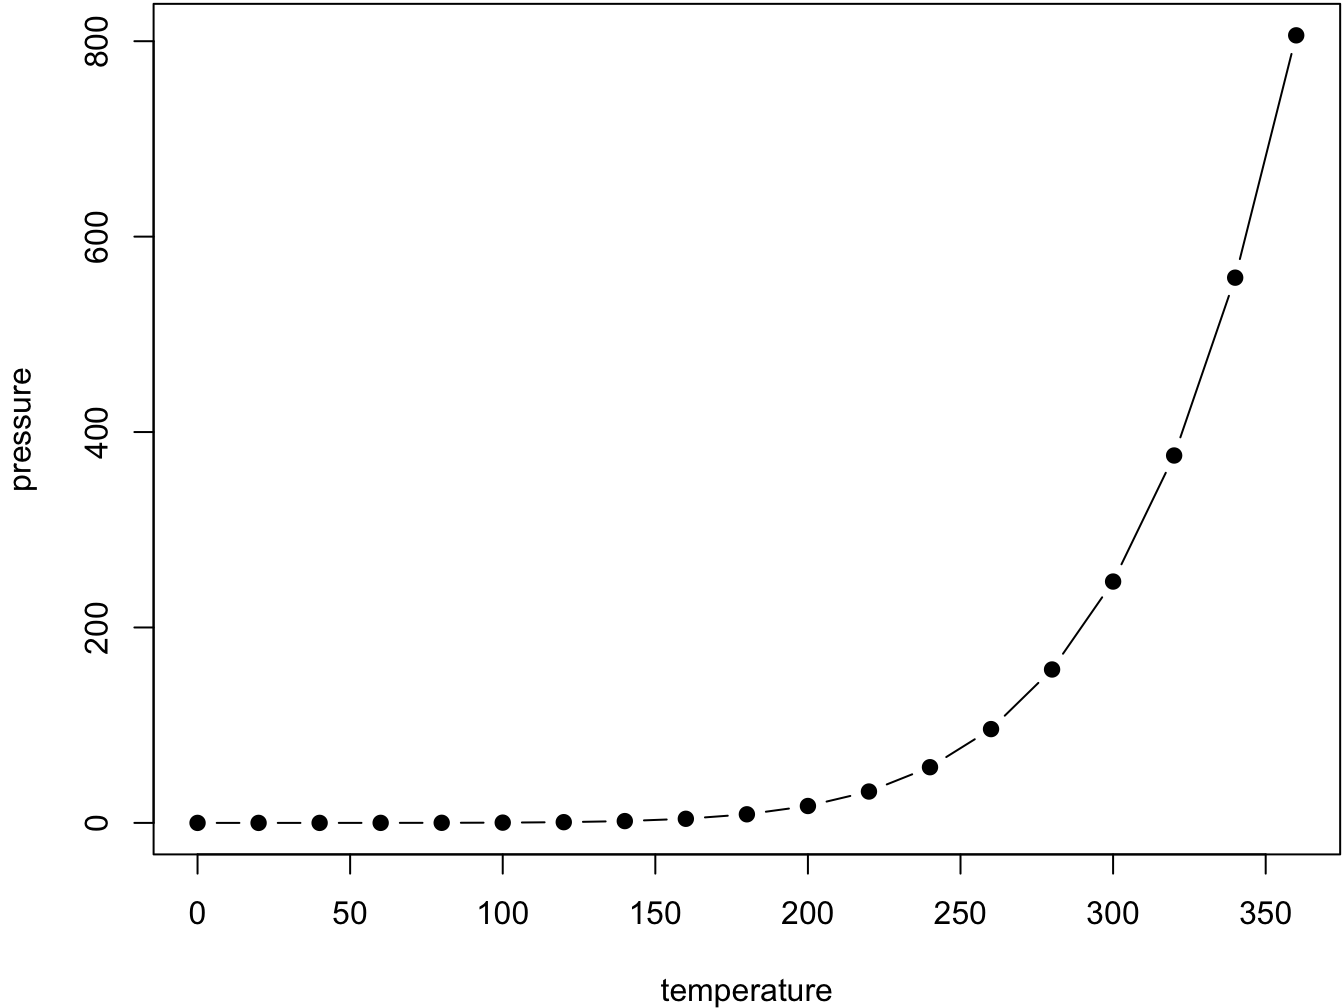
\includegraphics[width=0.8\linewidth]{Statistics-Book_files/figure-latex/nice-fig-1} 

}

\caption{Here is a nice figure!}\label{fig:nice-fig}
\end{figure}

Reference a figure by its code chunk label with the \texttt{fig:} prefix, e.g., see Figure \ref{fig:nice-fig}. Similarly, you can reference tables generated from \texttt{knitr::kable()}, e.g., see Table \ref{tab:nice-tab}.

\begin{Shaded}
\begin{Highlighting}[]
\NormalTok{knitr}\SpecialCharTok{::}\FunctionTok{kable}\NormalTok{(}
  \FunctionTok{head}\NormalTok{(iris, }\DecValTok{20}\NormalTok{), }\AttributeTok{caption =} \StringTok{\textquotesingle{}Here is a nice table!\textquotesingle{}}\NormalTok{,}
  \AttributeTok{booktabs =} \ConstantTok{TRUE}
\NormalTok{)}
\end{Highlighting}
\end{Shaded}

\begin{table}

\caption{\label{tab:nice-tab}Here is a nice table!}
\centering
\begin{tabular}[t]{rrrrl}
\toprule
Sepal.Length & Sepal.Width & Petal.Length & Petal.Width & Species\\
\midrule
5.1 & 3.5 & 1.4 & 0.2 & setosa\\
4.9 & 3.0 & 1.4 & 0.2 & setosa\\
4.7 & 3.2 & 1.3 & 0.2 & setosa\\
4.6 & 3.1 & 1.5 & 0.2 & setosa\\
5.0 & 3.6 & 1.4 & 0.2 & setosa\\
\addlinespace
5.4 & 3.9 & 1.7 & 0.4 & setosa\\
4.6 & 3.4 & 1.4 & 0.3 & setosa\\
5.0 & 3.4 & 1.5 & 0.2 & setosa\\
4.4 & 2.9 & 1.4 & 0.2 & setosa\\
4.9 & 3.1 & 1.5 & 0.1 & setosa\\
\addlinespace
5.4 & 3.7 & 1.5 & 0.2 & setosa\\
4.8 & 3.4 & 1.6 & 0.2 & setosa\\
4.8 & 3.0 & 1.4 & 0.1 & setosa\\
4.3 & 3.0 & 1.1 & 0.1 & setosa\\
5.8 & 4.0 & 1.2 & 0.2 & setosa\\
\addlinespace
5.7 & 4.4 & 1.5 & 0.4 & setosa\\
5.4 & 3.9 & 1.3 & 0.4 & setosa\\
5.1 & 3.5 & 1.4 & 0.3 & setosa\\
5.7 & 3.8 & 1.7 & 0.3 & setosa\\
5.1 & 3.8 & 1.5 & 0.3 & setosa\\
\bottomrule
\end{tabular}
\end{table}

You can write citations, too. For example, we are using the \textbf{bookdown} package \citep{R-bookdown} in this sample book, which was built on top of R Markdown and \textbf{knitr} \citep{xie2015}.

\#Front Matter from Example

This is a \emph{sample} book written in \textbf{Markdown}. You can use anything that Pandoc's Markdown supports, e.g., a math equation \(a^2 + b^2 = c^2\).

The \textbf{bookdown} package can be installed from CRAN or Github:

\begin{Shaded}
\begin{Highlighting}[]
\FunctionTok{install.packages}\NormalTok{(}\StringTok{"bookdown"}\NormalTok{)}
\CommentTok{\# or the development version}
\CommentTok{\# devtools::install\_github("rstudio/bookdown")}
\end{Highlighting}
\end{Shaded}

Remember each Rmd file contains one and only one chapter, and a chapter is defined by the first-level heading \texttt{\#}.

To compile this example to PDF, you need XeLaTeX. You are recommended to install TinyTeX (which includes XeLaTeX): \url{https://yihui.org/tinytex/}.

  \bibliography{book.bib,packages.bib}

\end{document}
